% If you want 16:9 add [aspectratio=169] before {beamer}
% Otherwise by default, it is 4:3 
\documentclass[aspectratio=169]{beamer}%
% Closing navigation
\setbeamertemplate{navigation symbols}{}%
% Theme
\usetheme{Boadilla}%
% Code listings
\usepackage{listings}%
% UTF8
\usepackage[utf8]{inputenc}%
% Color pack
\usepackage{xcolor}%
% For combination notation, math library
\usepackage{amsmath}
% For multicolumn items
\usepackage{multicol}
% For links and navigation
\usepackage{hyperref}

% Enumeration and Itemization settings
\setbeamertemplate{itemize items}[square]
\setbeamertemplate{enumerate items}[default]%

% Beamer Colors
\definecolor{footblue}{RGB}{0,84,160}%
\definecolor{footaqua}{RGB}{0,138,203}%
\setbeamercolor{author in head/foot}{fg=white, bg=footaqua}%
\setbeamercolor{title in head/foot}{fg=white, bg=footblue}%
\setbeamercolor{date in head/foot}{fg=white, bg=footaqua}%
\setbeamercolor{frametitle}{fg=footblue, bg=white}%
\setbeamercolor{titlelike}{fg=footblue}%
\setbeamercolor{itemize item}{fg=footblue}%
\setbeamercolor{itemize subitem}{fg=footblue}%
\setbeamercolor{itemize subsubitem}{fg=footblue}%
\setbeamercolor{itemize subsubsubitem}{fg=footblue}%
\setbeamercolor{enumerate item}{fg=footblue}%
\setbeamercolor{enumerate subitem}{fg=footblue}%
\setbeamercolor{enumerate subsubitem}{fg=footblue}%
\setbeamercolor{enumerate subsubsubitem}{fg=footblue}%
\setbeamercolor{caption name}{fg=footblue}%

% Title settings
\title{ALGO-101}%
\subtitle{Week 5 - Graphs and Trees}%
\author{Fatih Baskın}%
\date{November 2022}%
\institute{ITU ACM}%

% Footline settings
\defbeamertemplate*{footline}{Boadilla}%
{%
    \leavevmode%
    \hbox{%
        \begin{beamercolorbox}[wd=.225\paperwidth,ht=2.25ex,dp=1ex,center]{author in head/foot}%
            \usebeamerfont{author in head/foot}\insertshortauthor%
        \end{beamercolorbox}%
        \begin{beamercolorbox}[wd=.55\paperwidth,ht=2.25ex,dp=1ex,center]{title in head/foot}%
            \usebeamerfont{title in head/foot}\insertshorttitle {} \insertsubtitle
        \end{beamercolorbox}%
        \begin{beamercolorbox}[wd=.225\paperwidth,ht=2.25ex,dp=1ex,right]{date in head/foot}%
            \usebeamerfont{date in head/foot}\insertshortdate{}\hspace*{2em}%
            \insertframenumber{} / \inserttotalframenumber\hspace*{2ex}%
        \end{beamercolorbox}}%
    \vskip0pt%
}%

% Code highlight colors
\definecolor{codegreen}{rgb}{0,0.6,0}%
\definecolor{codered}{rgb}{0.6,0,0}%
\definecolor{codegray}{rgb}{0.5,0.5,0.5}%
\definecolor{codepurple}{rgb}{0.58,0,0.82}%
\definecolor{backcolour}{rgb}{0.95,0.95,0.92}%

% Code highlight settings
\lstdefinestyle{mystyle}%
{%
    commentstyle=\color{codegreen},%
    keywordstyle=\color{blue},%
    numberstyle=\tiny\color{codegray},%
    stringstyle=\color{codered},%
    basicstyle=\ttfamily\footnotesize,%
    breakatwhitespace=false,%
    breaklines=true,%
    captionpos=b,%
    keepspaces=true,%
    numbers=left,%
    numbersep=5pt,%
    showspaces=false,%
    showstringspaces=false,%
    showtabs=false,%
    tabsize=4,%
    xleftmargin=12pt,%
}%
% Applying code highlight style
\lstset{style=mystyle}%

\begin{document}%

% Creating title page
\frame{\titlepage}%

\begin{frame}{Topics}
    % Text here
    Topics covered at week 5:
    % Itemized List
    \begin{itemize}%
        \item Graphs
            \begin{itemize}
                \item DFS and BFS
                \item Topological Sort
            \end{itemize}
        \item Trees
            \begin{itemize}%
                \item Tree Traversals
                \item Binary Search Tree
            \end{itemize}%
    \end{itemize}%
\end{frame}%

\begin{frame}{Graphs, Definitions}%
    \begin{columns}[T]%
        \begin{column}{.66\textwidth}%
            \begin{itemize}
                \item \textbf{Node} is a data element of a graph. Also called \textbf{vertex}.
                \item \textbf{Edge} is a line that connects two nodes.
                    \begin{itemize}
                        \item Shown as \textbf{ e = (v1, v2)}.
                        \item In this case, edge \textbf{e} is \textbf{incident} to nodes \textbf{v1} and \textbf{v2}.
                        \item Can be weighted, if so they are called \textbf{weighted edge}.
                        \item If graph is directed, they are called \textbf{arc}.
                    \end{itemize}
                \item \textbf{Adjacent} nodes are connected by an edge.
                \item \textbf{Self-loop} is an edge that connects a node to itself.
                \item Two nodes can be connected by more than one edges, these edges are called \textbf{parallel edges}.
                \item A \textbf{plain graph} does not contain any self-loops or parallel edges. If so, that graph is called \textbf{multigraph}.
            \end{itemize}
        \end{column}%
        \hfill
        \begin{column}{.30\textwidth}%
            \begin{figure}%
                \centering%
                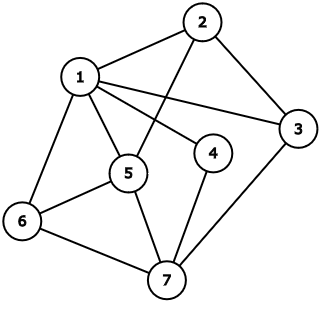
\includegraphics[width=.9\linewidth]{graph1.png}%
                \caption{A plain graph example}%
            \end{figure}%
        \end{column}%
    \end{columns}%
\end{frame}%

\begin{frame}{Graphs, Examples}%
    \begin{columns}[T]%
        \begin{column}{.32\textwidth}%
            \begin{figure}%
                \centering%
                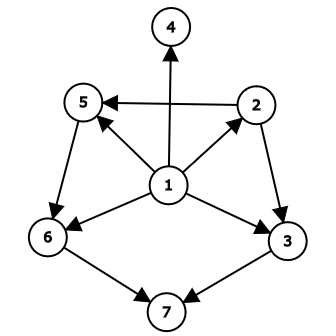
\includegraphics[width=.9\linewidth]{graph2.png}%
                \caption{Directed graph example}%
            \end{figure}%
        \end{column}%
        \hfill
        \begin{column}{.32\textwidth}%
            \begin{figure}%
                \centering%
                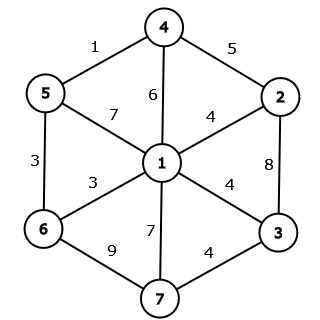
\includegraphics[width=.9\linewidth]{graph3.png}%
                \caption{Weighted graph example}%
            \end{figure}%
        \end{column}%
        \hfill
        \begin{column}{.32\textwidth}%
            \begin{figure}%
                \centering%
                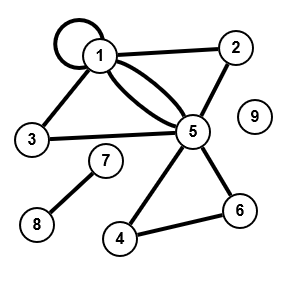
\includegraphics[width=.9\linewidth]{graph4.png}%
                \caption{Multigraph example}%
            \end{figure}%
        \end{column}%
    \end{columns}%
\end{frame}

\begin{frame}{Paths, Walks, Trails, Circuits, Cycles}
\begin{columns}[T]%
        \begin{column}{.66\textwidth}%
        \begin{itemize}
            \item \textbf{Walk} is a sequence of nodes and edges in a graph.
            \item \textbf{Trail} is a walk without visiting the same edge.
            \item \textbf{Circuit} is a trail that has the same node at the start and end.
            \item \textbf{Path} is a walk without visiting same node.
            \item \textbf{Cycle} is a circuit without visiting same node.
            \item \textbf{Spanning trail} covers all edges.
            \item \textbf{Spanning cycle} covers all nodes.
            \item \textbf{Euler graphs} contains closed spanning trail.
            \item \textbf{Hamilton graphs} contains a closed spanning path.
                \begin{itemize}
                    \item ref: \href{https://github.com/inzva/Algorithm-Program/tree/master/bundles}{\underline{inzva, 2018}}
                \end{itemize}
        \end{itemize}
        \end{column}%
        \hfill
        \begin{column}{.30\textwidth}%
            \begin{figure}%
                \centering%
                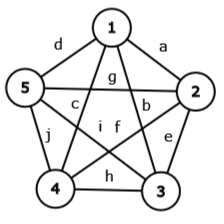
\includegraphics[width=.9\linewidth]{graph8.png}%
                \caption{Find paths, walks, trails, circuits, cycles}%
            \end{figure}%
        \end{column}%
    \end{columns}%
    
\end{frame}

\begin{frame}{Graphs, Definitions Cont.}%
    \begin{columns}[T]%
        \begin{column}{.66\textwidth}%
            \begin{itemize}
                \item \textbf{Degree} of a node means number of incident edges.
                    \begin{itemize}
                        \item $d_1$ = 6, $d_2$ = 2 ...
                        \item \textbf{In-degree} and \textbf{out-degree} for weighted graphs.
                    \end{itemize}
                \item \textbf{Connected graphs} have a path between every pair of nodes. 
                \item Disconnected graphs can be divided into \textbf{connected components}.
                    \begin{multicols}{3}                    
                        \begin{itemize}
                            \item 1, 2, 3, 4, 5, 6
                            \item 7, 8
                            \item 9
                        \end{itemize}
                    \end{multicols}
                \item \textbf{Distance} between nodes is the length/weight of shortest path between those nodes.
                \item Largest distance in graph is called \textbf{diameter} of graph.
            \end{itemize}
        \end{column}%
        \hfill
        \begin{column}{.30\textwidth}%
            \begin{figure}%
                \centering%
                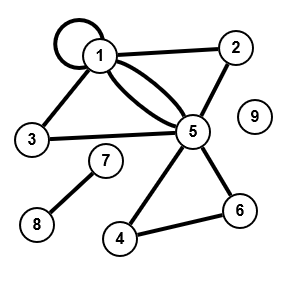
\includegraphics[width=.9\linewidth]{graph4.png}%
                \caption{Disconnected graph example}%
            \end{figure}%
        \end{column}%
    \end{columns}%
\end{frame}

\begin{frame}{Special Graphs}%
    \begin{columns}[T]%
        \begin{column}{.66\textwidth}%
            \begin{itemize}
            \item \textbf{Completely connected graph}s have an edge between every pair of nodes.
                \begin{itemize}
                    \item Number of nodes: n
                    \item Special name $K_n$                
                    \item Number of edges: $\binom{n}{k}$ = $\frac{n(n-1)}{2}$                    
                \end{itemize}
            \item \textbf{Tree} is a special type of graph.
                \begin{itemize}
                    \item Undirected,
                    \item Connected,
                    \item No cycles, exactly one path between every pair of nodes,
                    \item If number of nodes is n, number of edges are (n - 1).
                \end{itemize}
            \item \textbf{Bipartite graph} is a graph whose vertices can be divided into two disjoint and independent sets.
                \begin{itemize}
                    \item ref: \href{https://ninova.itu.edu.tr/tr/dersler/bilgisayar-bilisim-fakultesi/142/blg-112/ekkaynaklar?g118771}{\underline{Uyar et al., 2016}}
                \end{itemize}
            \item All nodes of a \textbf{regular graph} have the same degree.
                \begin{itemize}
                    \item \textbf{n-regular}: All nodes have degree n.
                \end{itemize}
            \end{itemize}
        \end{column}%
        \hfill
        \begin{column}{.30\textwidth}%
            \begin{figure}%
                \centering%
                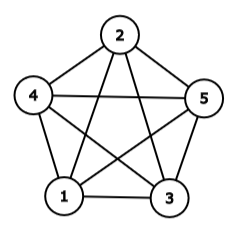
\includegraphics[width=.9\linewidth]{graph5.png}%
                \caption{Completely connected graph example, $K_5$}%
            \end{figure}%
        \end{column}%
    \end{columns}%
\end{frame}

\begin{frame}{Special Graphs, Examples}%
    \begin{columns}[T]%
        \begin{column}{.32\textwidth}%
            \begin{figure}%
                \centering%
                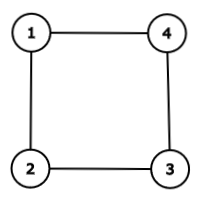
\includegraphics[width=.9\linewidth]{graph6.png}%
                \caption{2-regular graph example}%
            \end{figure}%
        \end{column}%
        \hfill
        \begin{column}{.32\textwidth}%
            \begin{figure}%
                \centering%
                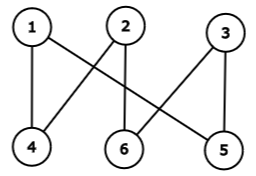
\includegraphics[width=.9\linewidth]{graph7.png}%
                \caption{Bipartite graph example}%
            \end{figure}%
        \end{column}%
        \hfill
        \begin{column}{.32\textwidth}%
            \begin{figure}%
                \centering%
                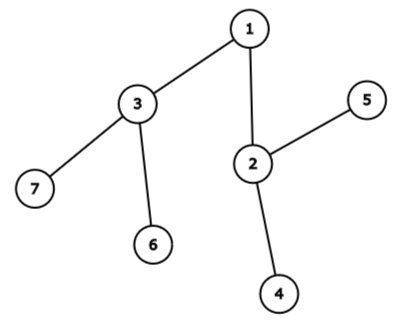
\includegraphics[width=.9\linewidth]{tree1.png}%
                \caption{Tree example}%
            \end{figure}%
        \end{column}%
    \end{columns}%
\end{frame}

\begin{frame}{Graph Representation, Adjacency Matrix}
    \begin{columns}
        \begin{column}{0.72\textwidth}
            \textbf{Matrix Representation}\\
            \begin{itemize}
                \item Store Boolean, adjacent or not?
                \item Store integer, weight.
            \end{itemize}
            \lstinputlisting[language = c++, linerange={4-14}]{graph_rep.cpp}
        \end{column}
        \hfill
        \begin{column}{0.24\textwidth}
            \begin{figure}
                \centering
                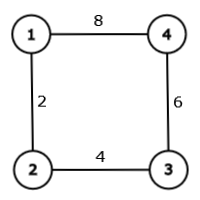
\includegraphics[width= 0.9\linewidth]{graph9.png}
                \caption{The graph represented in the code.}
            \end{figure}
        \end{column}
    \end{columns}
\end{frame}

\begin{frame}{Graph Representation, Adjacency List}
    \begin{columns}
        \begin{column}{0.72\textwidth}
            \textbf{Matrix Representation}\\
            \begin{itemize}
                \item Store adjacent nodes' numbers.
                \item Store \texttt{pair<\textcolor{blue}{int}, \color{blue}{int}>}, weight.
            \end{itemize}
            \lstinputlisting[language = c++, linerange={16-25}]{graph_rep.cpp}
        \end{column}
        \hfill
        \begin{column}{0.24\textwidth}
            \begin{figure}
                \centering
                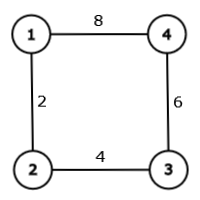
\includegraphics[width= 0.9\linewidth]{graph9.png}
                \caption{The graph represented in the code.}
            \end{figure}
        \end{column}
    \end{columns}
\end{frame}

\begin{frame}{Graph Exploration Methods}
    \begin{itemize}
        \item Two ways to explore a graph, \textbf{BFS} and \textbf{DFS}.
        \item Both do the same task using different methods.
        \item Requires a \textbf{starting node}, a \textbf{hash map} and adequate data structure (\textbf{queue or stack}).
        \item \textbf{BFS (Breadth First Search)}: Explore using a \textbf{queue}.            
        \item \textbf{DFS (Depth First Search)}: Explore using a \textbf{stack}.
        \item Both have time complexity \textbf{O(V + E)} and space complexity \textbf{O(V)}.
        \begin{itemize}
            \item V: number of nodes, E: number of edges.
        \end{itemize}
    \end{itemize}
\end{frame}

\begin{frame}{BFS (Breadth First Search)}
    \begin{itemize}
        \item From a starting node, explore all nodes level by level.
        \item First explore nodes one step away, then two step away...
        \item This logic implies an usage of a queue.
    \end{itemize}
    Its algorithm is basically:
    \begin{enumerate}
        \item Push starting node to queue and mark it as used.
        \item Take node \textbf{V} at the front of the queue. If the queue is empty, terminate.
        \item Push the unvisited nodes adjacent to \textbf{V} into the queue and mark them as used.
        \item Write down \textbf{V} and pop it from the queue.
        \item Jump to step 2.
    \end{enumerate}
\end{frame}

\begin{frame}{BFS Example Part 1}
    \begin{columns}
        \begin{column}{0.32\textwidth}
            \begin{figure}[!ht]
                \centering
                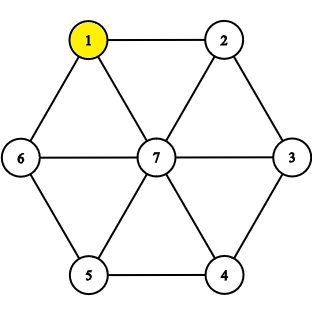
\includegraphics[width=0.9\linewidth]{bfs 1.png}
            \end{figure}
            \begin{table}[ht]
                \centering
                \begin{tabular}{l c}
                    Current node & -\\
                    Queue & 1 \\ 
                    Used nodes & 1\\
                    BFS & -
                \end{tabular}
            \end{table}
        \end{column}
        \hfill
        \begin{column}{0.32\textwidth}
            \begin{figure}[!ht]
                \centering
                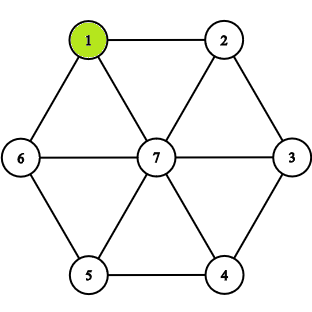
\includegraphics[width=0.9\linewidth]{bfs 2.png}
            \end{figure}
            \begin{table}[ht]
                \centering
                \begin{tabular}{l c}
                    Current node & 1\\
                    Queue & 1 \\ 
                    Used nodes & 1\\
                    BFS & -
                \end{tabular}
            \end{table}
        \end{column}
        \hfill
        \begin{column}{0.32\textwidth}
            \begin{figure}[!ht]
                \centering
                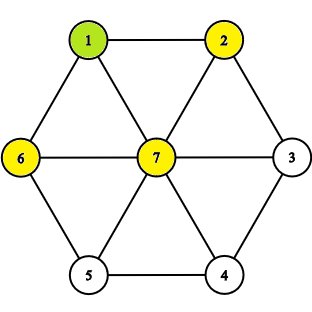
\includegraphics[width=0.9\linewidth]{bfs 3.png}
            \end{figure}
            \begin{table}[ht]
                \centering
                \begin{tabular}{l c}
                    Current node & 1\\
                    Queue & 1 2 7 6 \\ 
                    Used nodes & 1 2 6 7\\
                    BFS & -
                \end{tabular}
            \end{table}
        \end{column}
    \end{columns}
\end{frame}

\begin{frame}{BFS Example Part 2}
    \begin{columns}
        \begin{column}{0.32\textwidth}
            \begin{figure}[!ht]
                \centering
                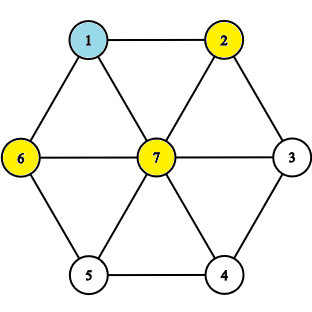
\includegraphics[width=0.9\linewidth]{bfs 4.png}
            \end{figure}
            \begin{table}[ht]
                \centering
                \begin{tabular}{l c}
                    Current node & -\\
                    Queue & 2 7 6 \\ 
                    Used nodes & 1 2 6 7\\
                    BFS & 1
                \end{tabular}
            \end{table}
        \end{column}
        \hfill
        \begin{column}{0.32\textwidth}
            \begin{figure}[!ht]
                \centering
                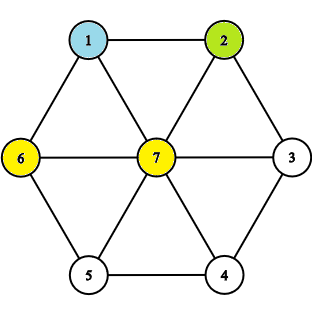
\includegraphics[width=0.9\linewidth]{bfs 5.png}
            \end{figure}
            \begin{table}[ht]
                \centering
                \begin{tabular}{l c}
                    Current node & 2\\
                    Queue & 2 7 6 \\ 
                    Used nodes & 1 2 6 7\\
                    BFS & 1
                \end{tabular}
            \end{table}
        \end{column}
        \hfill
        \begin{column}{0.32\textwidth}
            \begin{figure}[!ht]
                \centering
                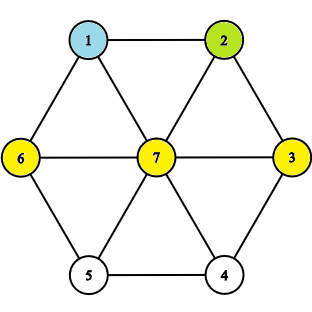
\includegraphics[width=0.9\linewidth]{bfs 6.png}
            \end{figure}
            \begin{table}[ht]
                \centering
                \begin{tabular}{l c}
                    Current node & 2\\
                    Queue & 2 7 6 3\\ 
                    Used nodes & 1 2 3 6 7\\
                    BFS & 1
                \end{tabular}
            \end{table}
        \end{column}
    \end{columns}
\end{frame}

\begin{frame}{BFS Example Part 3}
    \begin{columns}
        \begin{column}{0.32\textwidth}
            \begin{figure}[!ht]
                \centering
                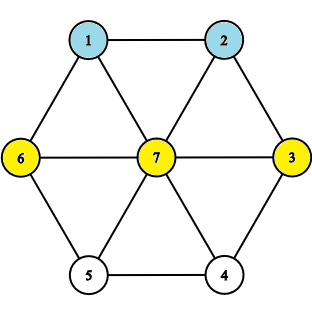
\includegraphics[width=0.9\linewidth]{bfs 7.png}
            \end{figure}
            \begin{table}[ht]
                \centering
                \begin{tabular}{l c}
                    Current node & -\\
                    Queue & 7 6 3\\ 
                    Used nodes & 1 2 3 6 7\\
                    BFS & 1 2
                \end{tabular}
            \end{table}
        \end{column}
        \hfill
        \begin{column}{0.32\textwidth}
            \begin{figure}[!ht]
                \centering
                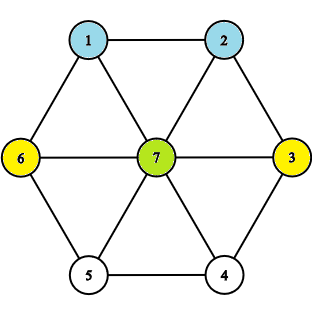
\includegraphics[width=0.9\linewidth]{bfs 8.png}
            \end{figure}
            \begin{table}[ht]
                \centering
                \begin{tabular}{l c}
                    Current node & 7\\
                    Queue & 7 6 3 \\ 
                    Used nodes & 1 2 3 6 7\\
                    BFS & 1 2
                \end{tabular}
            \end{table}
        \end{column}
        \hfill
        \begin{column}{0.32\textwidth}
            \begin{figure}[!ht]
                \centering
                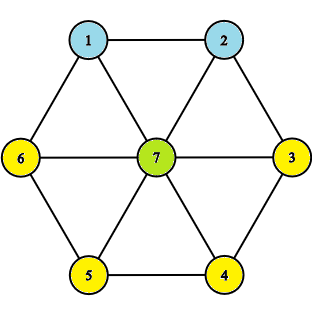
\includegraphics[width=0.9\linewidth]{bfs 9.png}
            \end{figure}
            \begin{table}[ht]
                \centering
                \begin{tabular}{l c}
                    Current node & 7\\
                    Queue & 7 6 3 4 5\\ 
                    Used nodes & ALL\\
                    BFS & 1 2
                \end{tabular}
            \end{table}
        \end{column}
    \end{columns}
\end{frame}

\begin{frame}{BFS Example Part 4}
    \begin{columns}
        \begin{column}{0.32\textwidth}
            \begin{figure}[!ht]
                \centering
                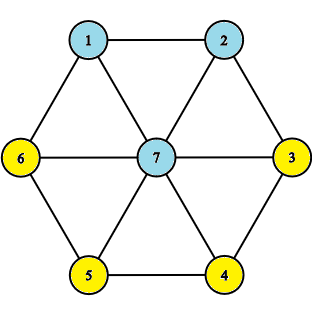
\includegraphics[width=0.9\linewidth]{bfs 10.png}
            \end{figure}
            \begin{table}[ht]
                \centering
                \begin{tabular}{l c}
                    Current node & -\\
                    Queue & 6 3 4 5\\ 
                    Used nodes & ALL\\
                    BFS & 1 2 7
                \end{tabular}
            \end{table}
        \end{column}
        \hfill
        \begin{column}{0.32\textwidth}
            \begin{figure}[!ht]
                \centering
                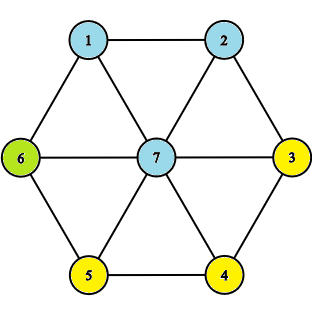
\includegraphics[width=0.9\linewidth]{bfs 11.png}
            \end{figure}
            \begin{table}[ht]
                \centering
                \begin{tabular}{l c}
                    Current node & 6\\
                    Queue & 6 3 4 5 \\ 
                    Used nodes & ALL\\
                    BFS & 1 2 7
                \end{tabular}
            \end{table}
        \end{column}
        \hfill
        \begin{column}{0.32\textwidth}
            \begin{figure}[!ht]
                \centering
                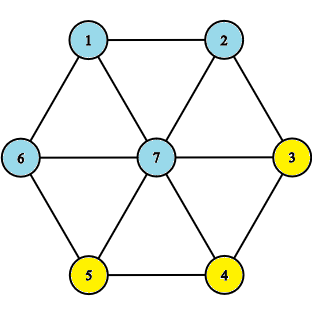
\includegraphics[width=0.9\linewidth]{bfs 12.png}
            \end{figure}
            \begin{table}[ht]
                \centering
                \begin{tabular}{l c}
                    Current node & -\\
                    Queue & 3 4 5\\ 
                    Used nodes & ALL\\
                    BFS & 1 2 7 6
                \end{tabular}
            \end{table}
        \end{column}
    \end{columns}
\end{frame}

\begin{frame}{BFS Example Part 5}
    \begin{columns}
        \begin{column}{0.32\textwidth}
            \begin{figure}[!ht]
                \centering
                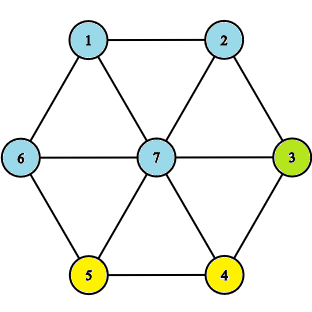
\includegraphics[width=0.9\linewidth]{bfs 13.png}
            \end{figure}
            \begin{table}[ht]
                \centering
                \begin{tabular}{l c}
                    Current node & 3\\
                    Queue & 3 4 5\\ 
                    Used nodes & ALL\\
                    BFS & 1 2 7 6
                \end{tabular}
            \end{table}
        \end{column}
        \hfill
        \begin{column}{0.32\textwidth}
            \begin{figure}[!ht]
                \centering
                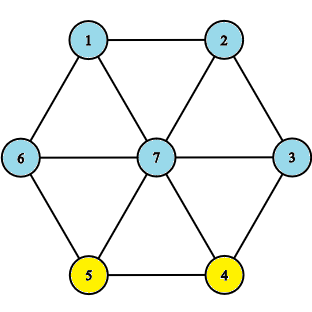
\includegraphics[width=0.9\linewidth]{bfs 14.png}
            \end{figure}
            \begin{table}[ht]
                \centering
                \begin{tabular}{l c}
                    Current node & -\\
                    Queue & 4 5\\ 
                    Used nodes & ALL\\
                    BFS & 1 2 7 6 3
                \end{tabular}
            \end{table}
        \end{column}
        \hfill
        \begin{column}{0.32\textwidth}
            \begin{figure}[!ht]
                \centering
                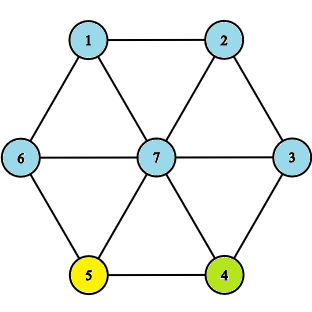
\includegraphics[width=0.9\linewidth]{bfs 15.png}
            \end{figure}
            \begin{table}[ht]
                \centering
                \begin{tabular}{l c}
                    Current node & 4\\
                    Queue & 4 5\\ 
                    Used nodes & ALL\\
                    BFS & 1 2 7 6 3
                \end{tabular}
            \end{table}
        \end{column}
    \end{columns}
\end{frame}

\begin{frame}{BFS Example Part 6}
    \begin{columns}
        \begin{column}{0.32\textwidth}
            \begin{figure}[!ht]
                \centering
                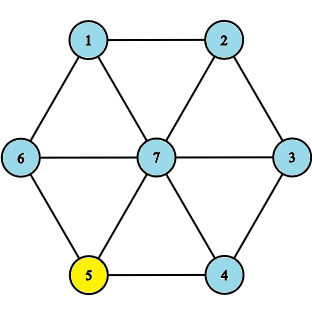
\includegraphics[width=0.9\linewidth]{bfs 16.png}
            \end{figure}
            \begin{table}[ht]
                \centering
                \begin{tabular}{l c}
                    Current node & -\\
                    Queue & 5\\ 
                    Used nodes & ALL\\
                    BFS & 1 2 7 6 3  4
                \end{tabular}
            \end{table}
        \end{column}
        \hfill
        \begin{column}{0.32\textwidth}
            \begin{figure}[!ht]
                \centering
                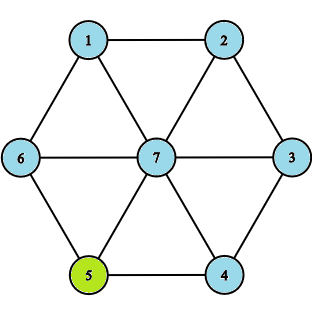
\includegraphics[width=0.9\linewidth]{bfs 17.png}
            \end{figure}
            \begin{table}[ht]
                \centering
                \begin{tabular}{l c}
                    Current node & 5\\
                    Queue & 5\\ 
                    Used nodes & ALL\\
                    BFS & 1 2 7 6 3 4
                \end{tabular}
            \end{table}
        \end{column}
        \hfill
        \begin{column}{0.32\textwidth}
            \begin{figure}[!ht]
                \centering
                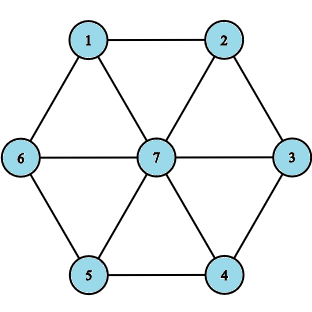
\includegraphics[width=0.9\linewidth]{bfs 18.png}
            \end{figure}
            \begin{table}[ht]
                \centering
                \begin{tabular}{l c}
                    Current node & -\\
                    Queue & -\\ 
                    Used nodes & ALL\\
                \end{tabular}
            \end{table}
            BFS complete: 1 2 7 6 3 4 5\\
        \end{column}
    \end{columns}
\end{frame}

\begin{frame}{BFS Code, Declerations}
    \begin{columns}
        \begin{column}{0.70\textwidth}
            \lstinputlisting[language = C++, linerange = {1 - 19}]{bfs_v1.cpp}%            
        \end{column}
        \hfill
        \begin{column}{0.25\textwidth}
            \begin{figure}[ht]
                \centering
                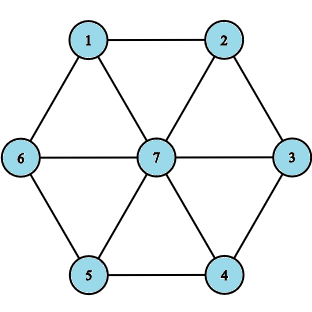
\includegraphics[width = .9\linewidth]{bfs 18.png}
                \caption{The graph used in the code}
            \end{figure}{}
        \end{column}
    \end{columns}    
\end{frame}

\begin{frame}{BFS Code, Operation}
    \begin{columns}
        \begin{column}{0.70\textwidth}
            \lstinputlisting[language = C++, linerange = {20 - 38}]{bfs_v1.cpp}%            
        \end{column}
        \hfill
        \begin{column}{0.25\textwidth}
            \begin{figure}[ht]
                \centering
                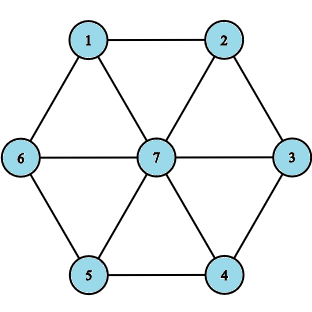
\includegraphics[width = .9\linewidth]{bfs 18.png}
                \caption{The graph used in the code}
            \end{figure}{}
        \end{column}
    \end{columns}    
\end{frame}

\begin{frame}{BFS with Saving Node Level}
    \lstinputlisting[language = C++, linerange = {18 - 36}]{bfs_v2.cpp}%      
\end{frame}

\begin{frame}{DFS (Depth First Search)}
    \begin{itemize}
        \item From a starting node, explore to the furthest depth possible.
        \item Trackback to next unexplored branches until complete.
        \item This logic implies an usage of a stack.
        \item It is possible to implement DFS with iterative and recursive methods.
    \end{itemize}
    Its algorithm is basically:
    \begin{enumerate}
        \item Push starting node to stack.
        \item Save the top node and pop it from the stack. If the stack is empty, terminate.
        \item Push unvisited adjacent nodes to stack.
        \item If the current node is not visited, write it down and mark it as visited.
        \item Jump to step 2.
    \end{enumerate}
\end{frame}

\begin{frame}{DFS Example Part 1}
    \begin{columns}
        \begin{column}{0.32\textwidth}
            \begin{figure}[!ht]
                \centering
                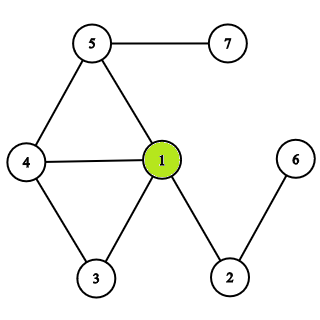
\includegraphics[width=0.9\linewidth]{dfs 1.png}
            \end{figure}
            \begin{table}[ht]
                \centering
                \begin{tabular}{l c}
                    Current node & 1\\
                    Stack & -\\ 
                    Used nodes & 1\\
                    DFS & -
                \end{tabular}
            \end{table}
        \end{column}
        \hfill
        \begin{column}{0.32\textwidth}
            \begin{figure}[!ht]
                \centering
                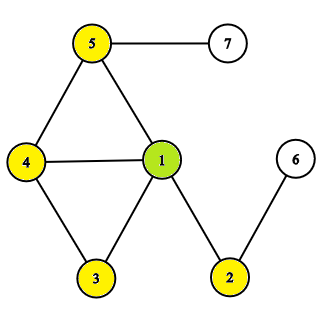
\includegraphics[width=0.9\linewidth]{dfs 2.png}
            \end{figure}
            \begin{table}[ht]
                \centering
                \begin{tabular}{l c}
                    Current node & 1\\
                    Stack & 2 3 4 5 \\ 
                    Used nodes & 1\\
                    DFS & -
                \end{tabular}
            \end{table}
        \end{column}
        \hfill
        \begin{column}{0.32\textwidth}
            \begin{figure}[!ht]
                \centering
                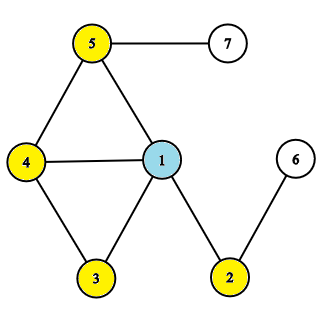
\includegraphics[width=0.9\linewidth]{dfs 3.png}
            \end{figure}
            \begin{table}[ht]
                \centering
                \begin{tabular}{l c}
                    Current node & -\\
                    Stack & 2 3 4 5\\ 
                    Used nodes & 1\\
                    DFS & 1
                \end{tabular}
            \end{table}
        \end{column}
    \end{columns}
\end{frame}

\begin{frame}{DFS Example Part 2}
    \begin{columns}
        \begin{column}{0.32\textwidth}
            \begin{figure}[!ht]
                \centering
                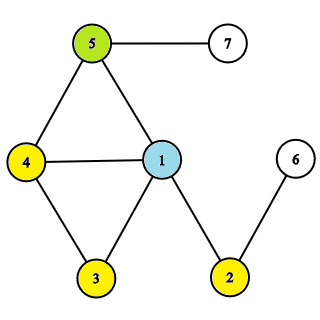
\includegraphics[width=0.9\linewidth]{dfs 4.png}
            \end{figure}
            \begin{table}[ht]
                \centering
                \begin{tabular}{l c}
                    Current node & 5\\
                    Stack & 2 3 4\\ 
                    Used nodes & 1 5\\
                    DFS & 1
                \end{tabular}
            \end{table}
        \end{column}
        \hfill
        \begin{column}{0.32\textwidth}
            \begin{figure}[!ht]
                \centering
                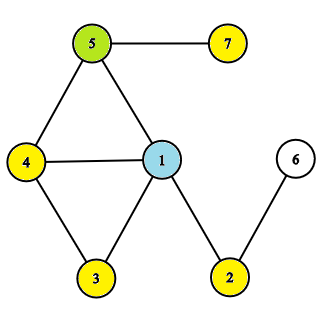
\includegraphics[width=0.9\linewidth]{dfs 5.png}
            \end{figure}
            \begin{table}[ht]
                \centering
                \begin{tabular}{l c}
                    Current node & 5\\
                    Stack & 2 3 4 4 7 \\ 
                    Used nodes & 1 5\\
                    DFS & 1
                \end{tabular}
            \end{table}
        \end{column}
        \hfill
        \begin{column}{0.32\textwidth}
            \begin{figure}[!ht]
                \centering
                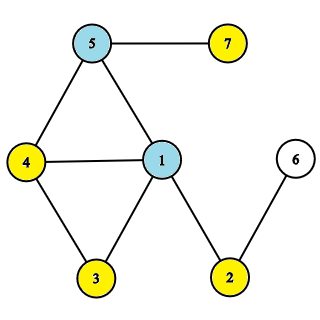
\includegraphics[width=0.9\linewidth]{dfs 6.png}
            \end{figure}
            \begin{table}[ht]
                \centering
                \begin{tabular}{l c}
                    Current node & -\\
                    Stack & 2 3 4 4 7\\ 
                    Used nodes & 1 5\\
                    DFS & 1 5
                \end{tabular}
            \end{table}
        \end{column}
    \end{columns}
\end{frame}

\begin{frame}{DFS Example Part 3}
    \begin{columns}
        \begin{column}{0.32\textwidth}
            \begin{figure}[!ht]
                \centering
                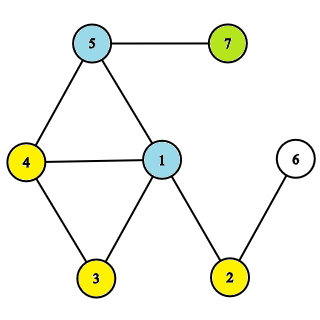
\includegraphics[width=0.9\linewidth]{dfs 7.png}
            \end{figure}
            \begin{table}[ht]
                \centering
                \begin{tabular}{l c}
                    Current node & 7\\
                    Stack & 2 3 4 4\\ 
                    Used nodes & 1 5 7\\
                    DFS & 1 5
                \end{tabular}
            \end{table}
        \end{column}
        \hfill
        \begin{column}{0.32\textwidth}
            \begin{figure}[!ht]
                \centering
                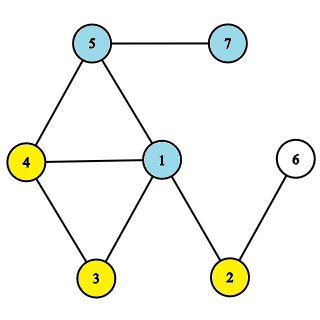
\includegraphics[width=0.9\linewidth]{dfs 8.png}
            \end{figure}
            \begin{table}[ht]
                \centering
                \begin{tabular}{l c}
                    Current node & -\\
                    Stack & 2 3 4 4\\ 
                    Used nodes & 1 5 7\\
                    DFS & 1 5 7
                \end{tabular}
            \end{table}
        \end{column}
        \hfill
        \begin{column}{0.32\textwidth}
            \begin{figure}[!ht]
                \centering
                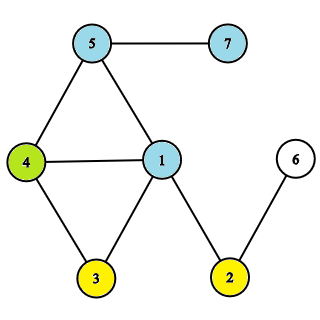
\includegraphics[width=0.9\linewidth]{dfs 9.png}
            \end{figure}
            \begin{table}[ht]
                \centering
                \begin{tabular}{l c}
                    Current node & 4\\
                    Stack & 2 3 4\\ 
                    Used nodes & 1 4 5 7\\
                    DFS & 1 5 7
                \end{tabular}
            \end{table}
        \end{column}
    \end{columns}
\end{frame}

\begin{frame}{DFS Example Part 4}
    \begin{columns}
        \begin{column}{0.32\textwidth}
            \begin{figure}[!ht]
                \centering
                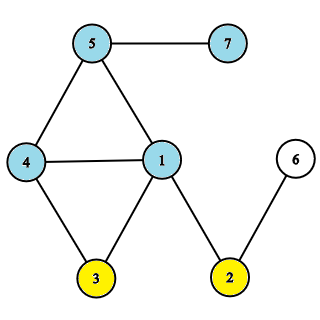
\includegraphics[width=0.9\linewidth]{dfs 10.png}
            \end{figure}
            \begin{table}[ht]
                \centering
                \begin{tabular}{l c}
                    Current node & -\\
                    Stack & 2 3 4 3\\ 
                    Used nodes & 1 4 5 7\\
                    DFS & 1 5 7 4
                \end{tabular}
            \end{table}
        \end{column}
        \hfill
        \begin{column}{0.32\textwidth}
            \begin{figure}[!ht]
                \centering
                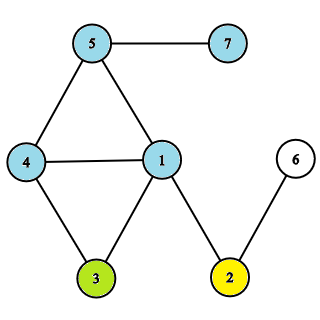
\includegraphics[width=0.9\linewidth]{dfs 11.png}
            \end{figure}
            \begin{table}[ht]
                \centering
                \begin{tabular}{l c}
                    Current node & 3\\
                    Stack & 2 3 4\\ 
                    Used nodes & 1 3 4 5 7\\
                    DFS & 1 5 7 4
                \end{tabular}
            \end{table}
        \end{column}
        \hfill
        \begin{column}{0.32\textwidth}
            \begin{figure}[!ht]
                \centering
                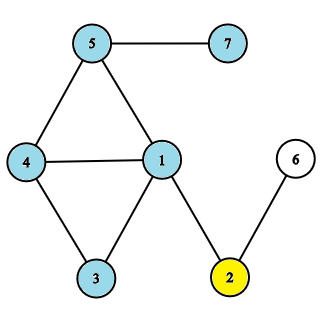
\includegraphics[width=0.9\linewidth]{dfs 12.png}
            \end{figure}
            \begin{table}[ht]
                \centering
                \begin{tabular}{l c}
                    Current node & -\\
                    Stack & 2 3 4\\ 
                    Used nodes & 1 3 4 5 7\\
                    DFS & 1 5 7 4 3 
                \end{tabular}
            \end{table}
        \end{column}
    \end{columns}
\end{frame}

\begin{frame}{DFS Example Part 5}
    \begin{columns}
        \begin{column}{0.32\textwidth}
            \begin{figure}[!ht]
                \centering
                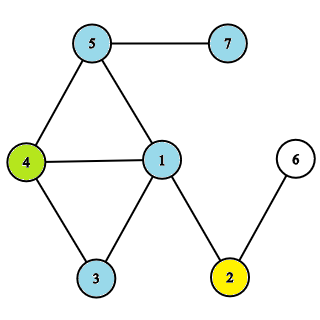
\includegraphics[width=0.9\linewidth]{dfs 13.png}
            \end{figure}
            \begin{table}[ht]
                \centering
                \begin{tabular}{l c}
                    Current node & 4\\
                    Stack & 2 3\\ 
                    Used nodes & 1 3 4 5 7\\
                    DFS & 1 5 7 4 3 
                \end{tabular}
            \end{table}
        \end{column}
        \hfill
        \begin{column}{0.32\textwidth}
            \begin{figure}[!ht]
                \centering
                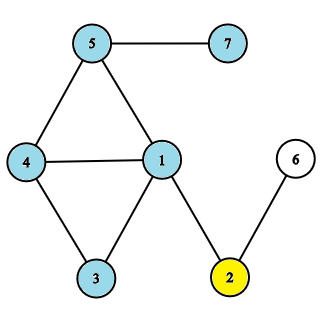
\includegraphics[width=0.9\linewidth]{dfs 14.png}
            \end{figure}
            \begin{table}[ht]
                \centering
                \begin{tabular}{l c}
                    Current node & -\\
                    Stack & 2 3\\ 
                    Used nodes & 1 3 4 5 7\\
                    DFS & 1 5 7 4 3 
                \end{tabular}
            \end{table}
        \end{column}
        \hfill
        \begin{column}{0.32\textwidth}
            \begin{figure}[!ht]
                \centering
                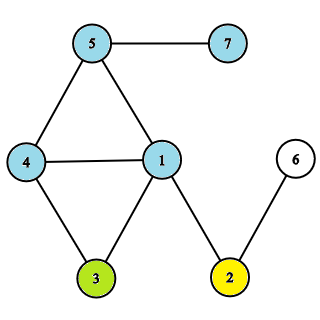
\includegraphics[width=0.9\linewidth]{dfs 15.png}
            \end{figure}
            \begin{table}[ht]
                \centering
                \begin{tabular}{l c}
                    Current node & 3\\
                    Stack & 2\\ 
                    Used nodes & 1 3 4 5 7\\
                    DFS & 1 5 7 4 3 
                \end{tabular}
            \end{table}
        \end{column}
    \end{columns}
\end{frame}

\begin{frame}{DFS Example Part 6}
    \begin{columns}
        \begin{column}{0.32\textwidth}
            \begin{figure}[!ht]
                \centering
                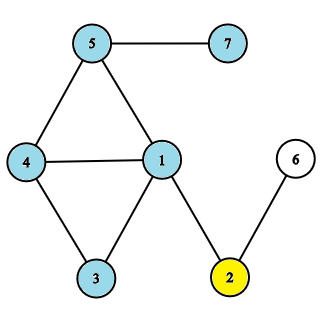
\includegraphics[width=0.9\linewidth]{dfs 16.png}
            \end{figure}
            \begin{table}[ht]
                \centering
                \begin{tabular}{l c}
                    Current node & -\\
                    Stack & 2\\ 
                    Used nodes & 1 3 4 5 7\\
                    DFS & 1 5 7 4 3 
                \end{tabular}
            \end{table}
        \end{column}
        \hfill
        \begin{column}{0.32\textwidth}
            \begin{figure}[!ht]
                \centering
                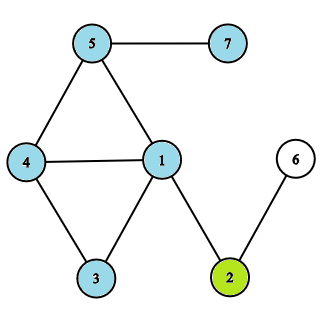
\includegraphics[width=0.9\linewidth]{dfs 17.png}
            \end{figure}
            \begin{table}[ht]
                \centering
                \begin{tabular}{l c}
                    Current node & 2\\
                    Stack & -\\ 
                    Used nodes & 1 2 3 4 5 7\\
                    DFS & 1 5 7 4 3 
                \end{tabular}
            \end{table}
        \end{column}
        \hfill
        \begin{column}{0.32\textwidth}
            \begin{figure}[!ht]
                \centering
                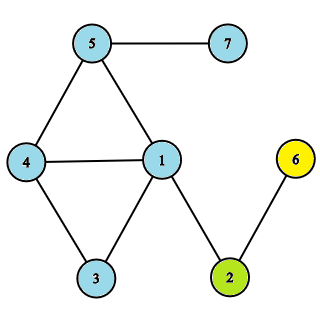
\includegraphics[width=0.9\linewidth]{dfs 18.png}
            \end{figure}
            \begin{table}[ht]
                \centering
                \begin{tabular}{l c}
                    Current node & 2\\
                    Stack & 6\\ 
                    Used nodes & 1 2 3 4 5 7\\
                    DFS & 1 5 7 4 3 
                \end{tabular}
            \end{table}
        \end{column}
    \end{columns}
\end{frame}

\begin{frame}{DFS Example Part 7}
    \begin{columns}
        \begin{column}{0.32\textwidth}
            \begin{figure}[!ht]
                \centering
                \includegraphics[width=0.9\linewidth]{dfs 19.png}
            \end{figure}
            \begin{table}[ht]
                \centering
                \begin{tabular}{l c}
                    Current node & -\\
                    Stack & 6\\ 
                    Used nodes & 1 2 3 4 5 7\\
                    DFS & 1 5 7 4 3 2 
                \end{tabular}
            \end{table}
        \end{column}
        \hfill
        \begin{column}{0.32\textwidth}
            \begin{figure}[!ht]
                \centering
                \includegraphics[width=0.9\linewidth]{dfs 20.png}
            \end{figure}
            \begin{table}[ht]
                \centering
                \begin{tabular}{l c}
                    Current node & 6\\
                    Stack & -\\ 
                    Used nodes & ALL\\
                    DFS & 1 5 7 4 3 2 
                \end{tabular}
            \end{table}
        \end{column}
        \hfill
        \begin{column}{0.32\textwidth}
            \begin{figure}[!ht]
                \centering
                \includegraphics[width=0.9\linewidth]{dfs 21.png}
            \end{figure}
            \begin{table}[ht]
                \centering
                \begin{tabular}{l c}
                    Current node & -\\
                    Stack & -\\ 
                    Used nodes & All\\
                \end{tabular}
            \end{table}
            DFS complete: 1 5 7 4 3 2 6
        \end{column}
    \end{columns}
\end{frame}

\begin{frame}{Iterative DFS Code, Declerations}
    \begin{columns}
        \begin{column}{0.70\textwidth}
            \lstinputlisting[language = c++, linerange = {1 - 19}]{dfs_v1.cpp}
        \end{column}
        \hfill
        \begin{column}{0.25\textwidth}
            \begin{figure}
                \centering
                \includegraphics[width = .9\linewidth]{dfs 21.png}
                \caption{The graph used in the code}
            \end{figure}
        \end{column}
    \end{columns}
\end{frame}

\begin{frame}{Iterative DFS Code, Operation}
    \begin{columns}
        \begin{column}{0.70\textwidth}
            \lstinputlisting[language = c++, linerange = {20 - 38}]{dfs_v1.cpp}
        \end{column}
        \hfill
        \begin{column}{0.25\textwidth}
            \begin{figure}
                \centering
                \includegraphics[width = .9\linewidth]{dfs 21.png}
                \caption{The graph used in the code}
            \end{figure}
        \end{column}
    \end{columns}
\end{frame}

\begin{frame}{Recursive DFS Code, Declerations}
    \begin{columns}
        \begin{column}{0.70\textwidth}
            \lstinputlisting[language = c++, linerange = {10 - 25}]{dfs_v2.cpp}
        \end{column}
        \hfill
        \begin{column}{0.25\textwidth}
            \begin{figure}
                \centering
                \includegraphics[width = .9\linewidth]{dfs 21.png}
                \caption{The graph used in the code}
            \end{figure}
        \end{column}
    \end{columns}
\end{frame}

\begin{frame}{Recursive DFS Code, DFS Function}
    \begin{columns}
        \begin{column}{0.70\textwidth}
            \lstinputlisting[language = c++, linerange = {27 - 38}]{dfs_v2.cpp}
            \begin{itemize}
                \item Note that recursive DFS would give correct but different answer compared to itterative DFS.
                \item 1 2 6 3 4 5 7
            \end{itemize}
        \end{column}
        \hfill
        \begin{column}{0.25\textwidth}
            \begin{figure}
                \centering
                \includegraphics[width = .9\linewidth]{dfs 21.png}
                \caption{The graph used in the code}
            \end{figure}
        \end{column}
    \end{columns}
\end{frame}

\begin{frame}{Comparison of BFS and DFS}
    \begin{table}[ht]
        \centering
        \begin{tabular}{|c||c|c|}
            \hline
             & DFS & BFS \\
             \hline
            Exploration order & Depth & Level\\
            Data structure & Stack & Queue\\
            Time complexity & O(V + E) & O(V + E)\\
            Space complexity & O(V) & O(V)\\
            Exploration tree & Narrow and long & Wide and short\\
            \hline
        \end{tabular}
        \caption{Ref: \href{https://iq.opengenus.org/dfs-vs-bfs/}{\underline{opengenus.org}}}
    \end{table}
\end{frame}

\begin{frame}{Topological Sort}
    \begin{itemize}
        \item With using a DFS, entirely traverse a \textbf{directed uncyclic graph (DAG)}.
        \item Use a stack to save the traversed nodes in a stack.
        \item Write down stack from top to bottom to store:
            \begin{itemize}
                \item For dependencies, install order,
                \item For lectures requiring previously taken courses, order of lectures that you should take,
                \item Order of tasks in task list in which certain tasks require previously completed tasks.
            \end{itemize}
        \item This algorithm fails if the graph is not a \textbf{DAG}.
            \begin{itemize}
                \item It is not the weakness of the algorithm, such graphs are impossible to topologically sort.
                \item If A requires B and B requires A to be done, it is impossible to do both tasks. 
            \end{itemize}
        \item Time complexity: \textbf{O(V + E)}
        \item Space complexity: \textbf{O(V)}
    \end{itemize}
\end{frame}

\begin{frame}{DAG and Not DAG Graph Examples}
\begin{columns}
    \begin{column}{.48\textwidth}
        \begin{figure}
            \centering
            \includegraphics[width = .9\linewidth]{graph10.png}
            \caption{Not a DAG, not topologically sort-able.}
        \end{figure}
    \end{column}
    \hfill
    \begin{column}{.48\textwidth}
        \begin{figure}
            \centering
            \includegraphics[width = .8\linewidth]{graph11.png}
            \caption{DAG, topologically sort-able}
        \end{figure}
    \end{column}
\end{columns}
\end{frame}

\begin{frame}{Topological Sort Example Part 1}
    \begin{columns}
        \begin{column}{.32\textwidth}
            \begin{figure}
                \centering
                \includegraphics[width = .9\linewidth]{topsort1.png}
                \caption{Topological Sort Stack: -empty-}
            \end{figure}
        \end{column}
        \hfill
        \begin{column}{.32\textwidth}
            \begin{figure}
                \centering
                \includegraphics[width = .9\linewidth]{topsort2.png}
                \caption{Topological Sort Stack: -empty-}
            \end{figure}            
        \end{column}
        \hfill
        \begin{column}{.32\textwidth}
            \begin{figure}
                \centering
                \includegraphics[width = .9\linewidth]{topsort3.png}
                \caption{Topological Sort Stack: -empty-}
            \end{figure}     
        \end{column}
    \end{columns}
\end{frame}

\begin{frame}{Topological Sort Example Part 2}
    \begin{columns}
        \begin{column}{.32\textwidth}
            \begin{figure}
                \centering
                \includegraphics[width = .9\linewidth]{topsort4.png}
                \caption{Topological Sort Stack: h}
            \end{figure}
        \end{column}
        \hfill
        \begin{column}{.32\textwidth}
            \begin{figure}
                \centering
                \includegraphics[width = .9\linewidth]{topsort5.png}
                \caption{Topological Sort Stack: h-g}
            \end{figure}                
        \end{column}
        \hfill
        \begin{column}{.32\textwidth}
            \begin{figure}
                \centering
                \includegraphics[width = .9\linewidth]{topsort6.png}
                \caption{Topological Sort Stack: h-g-a}
            \end{figure}
        \end{column}
    \end{columns}
\end{frame}

\begin{frame}{Topological Sort Example Part 3}
    \begin{columns}
        \begin{column}{.32\textwidth}
            \begin{figure}
                \centering
                \includegraphics[width = .9\linewidth]{topsort7.png}
                \caption{Topological Sort Stack: h-g-a}
            \end{figure}
        \end{column}
        \hfill
        \begin{column}{.32\textwidth}
            \begin{figure}
                \centering
                \includegraphics[width = .9\linewidth]{topsort8.png}
                \caption{Topological Sort Stack: h-g-a}
            \end{figure}
        \end{column}
        \hfill
        \begin{column}{.32\textwidth}
            \begin{figure}
                \centering
                \includegraphics[width = .9\linewidth]{topsort9.png}
                \caption{Topological Sort Stack: h-g-a-e}
            \end{figure}
        \end{column}
    \end{columns}
\end{frame}

\begin{frame}{Topological Sort Example Part 4}
    \begin{columns}
        \begin{column}{.32\textwidth}
            \begin{figure}
                \centering
                \includegraphics[width = .9\linewidth]{topsort10.png}
                \caption{Topological Sort Stack: h-g-a-e-c}
            \end{figure}
        \end{column}
        \hfill
        \begin{column}{.32\textwidth}
            \begin{figure}
                \centering
                \includegraphics[width = .9\linewidth]{topsort11.png}
                \caption{Topological Sort Stack: h-g-a-e-c-f}
            \end{figure}
        \end{column}
        \hfill
        \begin{column}{.32\textwidth}
            \begin{figure}
                \centering
                \includegraphics[width = .9\linewidth]{topsort12.png}
                \caption{Topological Sort Stack: h-g-a-e-c-f-b}
            \end{figure}
        \end{column}
    \end{columns}
\end{frame}

\begin{frame}{Topological Sort Recursive DFS Code}
    \lstinputlisting[language = c++, linerange = {14-24}]{topsort_v1.cpp}
\end{frame}

\begin{frame}{Topological Sort Function Call and Printing Stack}
    \lstinputlisting[language = c++, linerange = {30-40}]{topsort_v1.cpp}
\end{frame}

\begin{frame}{Tree Traversals}
    \begin{itemize}
        \item Trees are called complete m-ary if nodes have either \textbf{0} or \textbf{m} child nodes.
        \item \textbf{Height} of a tree is the longest path from the \textbf{root} of the tree and its \textbf{leaves.}
        \item Three ways to traverse a complete binary tree.
    \end{itemize}
    \begin{multicols}{3}
        \begin{itemize}
            \item Preorder traversal
            \item value, left, right
            \item Inorder traversal
            \item left, value, right
            \item Postorder traversal
            \item left, right, value
        \end{itemize}
    \end{multicols}
    \begin{itemize}
        \item Traversals are used to notate a tree.
        \item Using recursive functions to traverse.
        \item Complexity is \textbf{O(n + m)} but for trees, \textbf{m = n - 1} so complexity is \textbf{O(n)}.
        \item Space complexity is \textbf{O(1)}.
        \item \textbf{Note:} Postorder traversal is also known as \textbf{reverse Polish notation}.
    \end{itemize}    
\end{frame}

\begin{frame}{Tree Struct Code}
    Struct:
    \lstinputlisting[language = c++, linerange = {6-12}]{tree_traversal.cpp}
    Declaration:
    \lstinputlisting[language = c++, linerange = {50-56}]{tree_traversal.cpp}
\end{frame}

\begin{frame}{Preorder Traversal Example Part 1}
    \begin{columns}
        \begin{column}{0.32\textwidth}
            \begin{figure}
                \centering
                \includegraphics[width = .9\linewidth]{tree-pre 1.png}
                \caption{Preorder Traversal: -empty-}
            \end{figure}
        \end{column}
        \hfill
        \begin{column}{0.32\textwidth}
            \begin{figure}
                \centering
                \includegraphics[width = .9\linewidth]{tree-pre 2.png}
                \caption{Preorder Traversal: 1}
            \end{figure}
        \end{column}
        \hfill
        \begin{column}{0.32\textwidth}
            \begin{figure}
                \centering
                \includegraphics[width = .9\linewidth]{tree-pre 3.png}
                \caption{Preorder Traversal: 1}
            \end{figure}
        \end{column}
    \end{columns}
\end{frame}

\begin{frame}{Preorder Traversal Example Part 2}
    \begin{columns}
        \begin{column}{0.32\textwidth}
            \begin{figure}
                \centering
                \includegraphics[width = .9\linewidth]{tree-pre 4.png}
                \caption{Preorder Traversal: 1-2}
            \end{figure}
        \end{column}
        \hfill
        \begin{column}{0.32\textwidth}
            \begin{figure}
                \centering
                \includegraphics[width = .9\linewidth]{tree-pre 5.png}
                \caption{Preorder Traversal: 1-2}
            \end{figure}
        \end{column}
        \hfill
        \begin{column}{0.32\textwidth}
            \begin{figure}
                \centering
                \includegraphics[width = .9\linewidth]{tree-pre 6.png}
                \caption{Preorder Traversal: 1-2-4}
            \end{figure}
        \end{column}
    \end{columns}
\end{frame}

\begin{frame}{Preorder Traversal Example Part 3}
    \begin{columns}
        \begin{column}{0.32\textwidth}
            \begin{figure}
                \centering
                \includegraphics[width = .9\linewidth]{tree-pre 7.png}
                \caption{Preorder Traversal: 1-2-4}
            \end{figure}
        \end{column}
        \hfill
        \begin{column}{0.32\textwidth}
            \begin{figure}
                \centering
                \includegraphics[width = .9\linewidth]{tree-pre 8.png}
                \caption{Preorder Traversal: 1-2-4-5}
            \end{figure}
        \end{column}
        \hfill
        \begin{column}{0.32\textwidth}
            \begin{figure}
                \centering
                \includegraphics[width = .9\linewidth]{tree-pre 9.png}
                \caption{Preorder Traversal: 1-2-4-5}
            \end{figure}
        \end{column}
    \end{columns}
\end{frame}

\begin{frame}{Preorder Traversal Example Part 4}
    \begin{columns}
        \begin{column}{0.32\textwidth}
            \begin{figure}
                \centering
                \includegraphics[width = .9\linewidth]{tree-pre 10.png}
                \caption{Preorder Traversal: 1-2-4-5-3}
            \end{figure}
        \end{column}
        \hfill
        \begin{column}{0.32\textwidth}
            \begin{figure}
                \centering
                \includegraphics[width = .9\linewidth]{tree-pre 11.png}
                \caption{Preorder Traversal: 1-2-4-5-3}
            \end{figure}
        \end{column}
        \hfill
        \begin{column}{0.32\textwidth}
            \begin{figure}
                \centering
                \includegraphics[width = .9\linewidth]{tree-pre 12.png}
                \caption{Preorder Traversal: 1-2-4-5-3-6}
            \end{figure}
        \end{column}
    \end{columns}
\end{frame}

\begin{frame}{Preorder Traversal Example Part 5}
    \begin{columns}
        \begin{column}{0.32\textwidth}
            \begin{figure}
                \centering
                \includegraphics[width = .9\linewidth]{tree-pre 13.png}
                \caption{Preorder Traversal: 1-2-4-5-3-6}
            \end{figure}
        \end{column}
        \hfill
        \begin{column}{0.32\textwidth}
            \begin{figure}
                \centering
                \includegraphics[width = .9\linewidth]{tree-pre 14.png}
                \caption{Preorder Traversal: 1-2-4-5-3-6-7}
            \end{figure}
        \end{column}
    \end{columns}
\end{frame}

\begin{frame}{Preorder Traversal Code}
    Recursive function:
    \lstinputlisting[language = c++, linerange = {25-34}]{tree_traversal.cpp}
    Function call:
    \lstinputlisting[language = c++, linerange = {57-59}]{tree_traversal.cpp}
\end{frame}

\begin{frame}{Inorder Traversal Example Part 1}
    \begin{columns}
        \begin{column}{0.32\textwidth}
            \begin{figure}
                \centering
                \includegraphics[width = .9\linewidth]{tree-in 1.png}
                \caption{Preorder Traversal: -empty-}
            \end{figure}
        \end{column}
        \hfill
        \begin{column}{0.32\textwidth}
            \begin{figure}
                \centering
                \includegraphics[width = .9\linewidth]{tree-in 2.png}
                \caption{Inorder Traversal: -empty-}
            \end{figure}
        \end{column}
        \hfill
        \begin{column}{0.32\textwidth}
            \begin{figure}
                \centering
                \includegraphics[width = .9\linewidth]{tree-in 3.png}
                \caption{Inorder Traversal: -empty-}
            \end{figure}
        \end{column}
    \end{columns}
\end{frame}

\begin{frame}{Inorder Traversal Example Part 2}
    \begin{columns}
        \begin{column}{0.32\textwidth}
            \begin{figure}
                \centering
                \includegraphics[width = .9\linewidth]{tree-in 4.png}
                \caption{Inorder Traversal: 4}
            \end{figure}
        \end{column}
        \hfill
        \begin{column}{0.32\textwidth}
            \begin{figure}
                \centering
                \includegraphics[width = .9\linewidth]{tree-in 5.png}
                \caption{Inorder Traversal: 4}
            \end{figure}
        \end{column}
        \hfill
        \begin{column}{0.32\textwidth}
            \begin{figure}
                \centering
                \includegraphics[width = .9\linewidth]{tree-in 6.png}
                \caption{Inorder Traversal: 4-2}
            \end{figure}
        \end{column}
    \end{columns}
\end{frame}

\begin{frame}{Inorder Traversal Example Part 3}
    \begin{columns}
        \begin{column}{0.32\textwidth}
            \begin{figure}
                \centering
                \includegraphics[width = .9\linewidth]{tree-in 7.png}
                \caption{Inorder Traversal: 4-2}
            \end{figure}
        \end{column}
        \hfill
        \begin{column}{0.32\textwidth}
            \begin{figure}
                \centering
                \includegraphics[width = .9\linewidth]{tree-in 8.png}
                \caption{Inorder Traversal: 4-2-5}
            \end{figure}
        \end{column}
        \hfill
        \begin{column}{0.32\textwidth}
            \begin{figure}
                \centering
                \includegraphics[width = .9\linewidth]{tree-in 9.png}
                \caption{Inorder Traversal: 4-2-5}
            \end{figure}
        \end{column}
    \end{columns}
\end{frame}

\begin{frame}{Inorder Traversal Example Part 4}
    \begin{columns}
        \begin{column}{0.32\textwidth}
            \begin{figure}
                \centering
                \includegraphics[width = .9\linewidth]{tree-in 10.png}
                \caption{Inorder Traversal: 4-2-5-1}
            \end{figure}
        \end{column}
        \hfill
        \begin{column}{0.32\textwidth}
            \begin{figure}
                \centering
                \includegraphics[width = .9\linewidth]{tree-in 11.png}
                \caption{Inorder Traversal: 4-2-5-1}
            \end{figure}
        \end{column}
        \hfill
        \begin{column}{0.32\textwidth}
            \begin{figure}
                \centering
                \includegraphics[width = .9\linewidth]{tree-in 12.png}
                \caption{Inorder Traversal: 4-2-5-1}
            \end{figure}
        \end{column}
    \end{columns}
\end{frame}

\begin{frame}{Inorder Traversal Example Part 5}
    \begin{columns}
        \begin{column}{0.32\textwidth}
            \begin{figure}
                \centering
                \includegraphics[width = .9\linewidth]{tree-in 13.png}
                \caption{Inorder Traversal: 4-2-5-1-6}
            \end{figure}
        \end{column}
        \hfill
        \begin{column}{0.32\textwidth}
            \begin{figure}
                \centering
                \includegraphics[width = .9\linewidth]{tree-in 14.png}
                \caption{Inorder Traversal: 4-2-5-1-6}
            \end{figure}
        \end{column}
        \hfill
        \begin{column}{0.32\textwidth}
            \begin{figure}
                \centering
                \includegraphics[width = .9\linewidth]{tree-in 15.png}
                \caption{Inorder Traversal: 4-2-5-1-6-3}
            \end{figure}
        \end{column}
    \end{columns}
\end{frame}

\begin{frame}{Inorder Traversal Example Part 6}
    \begin{columns}
        \begin{column}{0.32\textwidth}
            \begin{figure}
                \centering
                \includegraphics[width = .9\linewidth]{tree-in 16.png}
                \caption{Inorder Traversal:  4-2-5-1-6-3}
            \end{figure}
        \end{column}
        \hfill
        \begin{column}{0.32\textwidth}
            \begin{figure}
                \centering
                \includegraphics[width = .9\linewidth]{tree-in 17.png}
                \caption{Inorder Traversal:  4-2-5-1-6-3-7}
            \end{figure}
        \end{column}
    \end{columns}
\end{frame}

\begin{frame}{Inorder Traversal Code}
    Recursive function:
    \lstinputlisting[language = c++, linerange = {14-23}]{tree_traversal.cpp}
    Function call:
    \lstinputlisting[language = c++, linerange = {60-62}]{tree_traversal.cpp}
\end{frame}

\begin{frame}{Postorder Traversal Example Part 1}
    \begin{columns}
        \begin{column}{0.32\textwidth}
            \begin{figure}
                \centering
                \includegraphics[width = .9\linewidth]{tree-post 1.png}
                \caption{Postorder Traversal: -empty-}
            \end{figure}
        \end{column}
        \hfill
        \begin{column}{0.32\textwidth}
            \begin{figure}
                \centering
                \includegraphics[width = .9\linewidth]{tree-post 2.png}
                \caption{Postorder Traversal: -empty-}
            \end{figure}
        \end{column}
        \hfill
        \begin{column}{0.32\textwidth}
            \begin{figure}
                \centering
                \includegraphics[width = .9\linewidth]{tree-post 3.png}
                \caption{Postorder Traversal: -empty-}
            \end{figure}
        \end{column}
    \end{columns}
\end{frame}

\begin{frame}{Postorder Traversal Example Part 2}
    \begin{columns}
        \begin{column}{0.32\textwidth}
            \begin{figure}
                \centering
                \includegraphics[width = .9\linewidth]{tree-post 4.png}
                \caption{Postorder Traversal: 4}
            \end{figure}
        \end{column}
        \hfill
        \begin{column}{0.32\textwidth}
            \begin{figure}
                \centering
                \includegraphics[width = .9\linewidth]{tree-post 5.png}
                \caption{Postorder Traversal: 4}
            \end{figure}
        \end{column}
        \hfill
        \begin{column}{0.32\textwidth}
            \begin{figure}
                \centering
                \includegraphics[width = .9\linewidth]{tree-post 6.png}
                \caption{Postorder Traversal: 4}
            \end{figure}
        \end{column}
    \end{columns}
\end{frame}

\begin{frame}{Postorder Traversal Example Part 3}
    \begin{columns}
        \begin{column}{0.32\textwidth}
            \begin{figure}
                \centering
                \includegraphics[width = .9\linewidth]{tree-post 7.png}
                \caption{Postorder Traversal: 4-5}
            \end{figure}
        \end{column}
        \hfill
        \begin{column}{0.32\textwidth}
            \begin{figure}
                \centering
                \includegraphics[width = .9\linewidth]{tree-post 8.png}
                \caption{Postorder Traversal: 4-5}
            \end{figure}
        \end{column}
        \hfill
        \begin{column}{0.32\textwidth}
            \begin{figure}
                \centering
                \includegraphics[width = .9\linewidth]{tree-post 9.png}
                \caption{Postorder Traversal: 4-5-2}
            \end{figure}
        \end{column}
    \end{columns}
\end{frame}

\begin{frame}{Postorder Traversal Example Part 4}
    \begin{columns}
        \begin{column}{0.32\textwidth}
            \begin{figure}
                \centering
                \includegraphics[width = .9\linewidth]{tree-post 10.png}
                \caption{Postorder Traversal: 4-5-2}
            \end{figure}
        \end{column}
        \hfill
        \begin{column}{0.32\textwidth}
            \begin{figure}
                \centering
                \includegraphics[width = .9\linewidth]{tree-post 11.png}
                \caption{Postorder Traversal: 4-5-2}
            \end{figure}
        \end{column}
        \hfill
        \begin{column}{0.32\textwidth}
            \begin{figure}
                \centering
                \includegraphics[width = .9\linewidth]{tree-post 12.png}
                \caption{Postorder Traversal: 4-5-2}
            \end{figure}
        \end{column}
    \end{columns}
\end{frame}

\begin{frame}{Postorder Traversal Example Part 5}
    \begin{columns}
        \begin{column}{0.32\textwidth}
            \begin{figure}
                \centering
                \includegraphics[width = .9\linewidth]{tree-post 13.png}
                \caption{Postorder Traversal: 4-5-2-6}
            \end{figure}
        \end{column}
        \hfill
        \begin{column}{0.32\textwidth}
            \begin{figure}
                \centering
                \includegraphics[width = .9\linewidth]{tree-post 14.png}
                \caption{Postorder Traversal: 4-5-2-6}
            \end{figure}
        \end{column}
        \hfill
        \begin{column}{0.32\textwidth}
            \begin{figure}
                \centering
                \includegraphics[width = .9\linewidth]{tree-post 15.png}
                \caption{Postorder Traversal: 4-5-2-6}
            \end{figure}
        \end{column}
    \end{columns}
\end{frame}

\begin{frame}{Postorder Traversal Example Part 6}
    \begin{columns}
        \begin{column}{0.32\textwidth}
            \begin{figure}
                \centering
                \includegraphics[width = .9\linewidth]{tree-post 16.png}
                \caption{Postorder Traversal: 4-5-2-6-7}
            \end{figure}
        \end{column}
        \hfill
        \begin{column}{0.32\textwidth}
            \begin{figure}
                \centering
                \includegraphics[width = .9\linewidth]{tree-post 17.png}
                \caption{Postorder Traversal: 4-5-2-6-7}
            \end{figure}
        \end{column}
        \hfill
        \begin{column}{0.32\textwidth}
            \begin{figure}
                \centering
                \includegraphics[width = .9\linewidth]{tree-post 18.png}
                \caption{Postorder Traversal: 4-5-2-6-7-3}
            \end{figure}
        \end{column}
    \end{columns}
\end{frame}

\begin{frame}{Postorder Traversal Example Part 7}
    \begin{columns}
        \begin{column}{0.32\textwidth}
            \begin{figure}
                \centering
                \includegraphics[width = .9\linewidth]{tree-post 19.png}
                \caption{Postorder Traversal: 4-5-2-6-7-3}
            \end{figure}
        \end{column}
        \hfill
        \begin{column}{0.32\textwidth}
            \begin{figure}
                \centering
                \includegraphics[width = .9\linewidth]{tree-post 20.png}
                \caption{Postorder Traversal: 4-5-2-6-7-3-1}
            \end{figure}
        \end{column}
    \end{columns}
\end{frame}

\begin{frame}{Postorder Traversal Code}
    Recursive function:
    \lstinputlisting[language = c++, linerange = {36-45}]{tree_traversal.cpp}
    Function call:
    \lstinputlisting[language = c++, linerange = {63-65}]{tree_traversal.cpp}
\end{frame}

\begin{frame}{Binary Search Tree}
    \begin{itemize}
        \item In the form of the binary tree data structure.
        \item Values of left sub-tree $<$ node's value.
        \item Values of right sub-tree $>$ node's value.
        \item Left-most value is the smallest.
        \item Right-most value is the greatest.
        \item If traversed inorder, you get a sorted array.
        \item \textbf{Balanced BST}: Depth of the leaves differ at most by 1.
        \item It is possible to construct a BST from any traversal of the BST or from an array.
        \item In a BST, you can find an item in \textbf{O(logn)} complexity.
    \end{itemize}
\end{frame}

\begin{frame}{Binary Search Tree Examples}
    \begin{columns}
        \begin{column}{0.32\textwidth}
            \begin{figure}
                \centering
                \includegraphics[width = 0.9\linewidth]{u_bst.png}
                \caption{Unbalanced BST example}
            \end{figure}
        \end{column}
        \hfill
        \begin{column}{0.32\textwidth}
            \begin{figure}
                \centering
                \includegraphics[width = 0.9\linewidth]{b_bst.png}
                \caption{Balanced BST example}
            \end{figure}
        \end{column}
        \hfill
        \begin{column}{0.32\textwidth}
            \begin{figure}
                \centering
                \includegraphics[width = 0.9\linewidth]{not_bst.png}
                \caption{Invalid BST example}
            \end{figure}
        \end{column}
    \end{columns}
\end{frame}

\begin{frame}{Constructing a BST from Scratch Example}
    \begin{columns}
         \begin{column}{0.32\textwidth}
                \begin{figure}
                    \centering
                    \includegraphics[width = .9\linewidth]{const_bst1.png}
                    \caption{Midpoint(s): 5}
                \end{figure}
            \end{column}
            \hfill
            \begin{column}{0.32\textwidth}
                \begin{figure}
                    \centering
                    \includegraphics[width = .9\linewidth]{const_bst2.png}
                    \caption{Midpoint(s): 2, 7}
                \end{figure}
            \end{column}
            \hfill
            \begin{column}{0.32\textwidth}
                \begin{figure}
                    \centering
                    \includegraphics[width = .9\linewidth]{const_bst3.png}
                    \caption{Balanced BST constructed.}
                \end{figure}
            \end{column}
    \end{columns}
\end{frame}

\begin{frame}{Balanced BST Construction Code, Tree Struct and Function Call}
    \lstinputlisting[language = c++, linerange = {4-12, 14-14, 33-34}]{balanced_bst.cpp}
\end{frame}

\begin{frame}{Balanced BST Construction Code, Recursive Construction Code}
    \lstinputlisting[language = c++, linerange = {16-29}]{balanced_bst.cpp}
\end{frame}

\begin{frame}{BST Search Algorithm}
    \begin{itemize}
        \item One of the benefits of BST is the ease of searching an item.
        \item Rather than searching linearly in an array, search using divide \& conquer.
        \item \textbf{O(logn)} complexity in a tree, rather than \textbf{O(n)} in an array.
        \item There exists dynamically configurable BSTs but they are out of today's scope.
        \item Those are called red \& black trees.
    \end{itemize}
    \begin{enumerate}
        \item If current node pointer is a null pointer return false.
        \item If current value is equal to required, return level or true \& false.
        \item If required value is bigger than current value, go right. (Go back to step 1)
        \item If required value is smaller than current value, go left. (Go back to step 1)
    \end{enumerate}
\end{frame}

\begin{frame}{BST Search Example}
    \begin{columns}
         \begin{column}{0.32\textwidth}
             \begin{figure}[ht]
                 \centering
                 \includegraphics[width = 0.9\linewidth]{bst_src1.png}
             \end{figure}
             \begin{table}[ht]
                 \centering
                 \begin{tabular}{cc}
                    Target & 9\\
                    Value  & 4\\
                    Action & Go Right\\
                 \end{tabular}
             \end{table}
         \end{column}
         \hfill
         \begin{column}{0.32\textwidth}
             \begin{figure}[ht]
                 \centering
                 \includegraphics[width = 0.9\linewidth]{bst_src2.png}
             \end{figure}
             \begin{table}[ht]
                 \centering
                 \begin{tabular}{cc}
                    Target & 9\\
                    Value  & 6\\
                    Action & Go Right\\
                 \end{tabular}
             \end{table}
         \end{column}
         \hfill
         \begin{column}{0.32\textwidth}
             \begin{figure}[ht]
                 \centering
                 \includegraphics[width = 0.9\linewidth]{bst_src3.png}
             \end{figure}
             \begin{table}[ht]
                 \centering
                 \begin{tabular}{cc}
                    Target & 9\\
                    Value  & 7\\
                    Action & Go Right\\
                 \end{tabular}
             \end{table}
             After going right, function will encounter a null pointer therefore it will return either an \textbf{invalid level} or \textbf{false}.
         \end{column}
    \end{columns}
\end{frame}

\begin{frame}{BST Search Code}
    \lstinputlisting[language = c++, linerange = {16-26}]{bst_search.cpp}
\end{frame}

\begin{frame}{Example Questions}
    \begin{itemize}
        \item \href{https://leetcode.com/submissions/detail/761526188/}{\underline{Path Sum II}} \emph{(DFS \& Tree \& Recursion)}
        \item \href{https://leetcode.com/submissions/detail/761730196/}{\underline{Number of Provinces}} \emph{(DFS)}
        \item \href{https://leetcode.com/submissions/detail/811277616/}{\underline{Course Schedule}} \emph{(Topological Sort)}
        \item \href{https://leetcode.com/submissions/detail/751458695/}{\underline{Convert Sorted Array to BST}} \emph{(Binary Search Tree)}
        \item \href{https://leetcode.com/submissions/detail/787225539/}{\underline{Validate Binary Search Tree}} \emph{(BST \& Tree Traversal)}
    \end{itemize}
\end{frame}

\end{document}%
